\section{Secondo metodo (2010)}
\subsection{Panoramica del metodo}\begin{frame}\frametitle{Panoramica del metodo}
Questo articolo\cite{2010} scritto nel 2010 e pubblicato in Analytical Chemistry {\bf tratta principalmente l'analisi strumentale}.
\pause

Viene utilizzato un metodo di purificazione particolarmente veloce e semplice per dimostrare il funzionamento del metodo anche in presenza di residui di interferenti.
\pause

La validazione del metodo viene effettuata {\bf comparando i risultati con il metodo di riferimento HRGC/HRMS} specificato in JIS K 0311 ed  {\bf analizzando materiali di riferimento certificati}.

Vengono fatti continui riferimenti al documento JIS K 0311 che è disponibile solo dietro pagamento.

\end{frame}

\subsubsection{Assicurazione della sicurezza nel laboratorio}\begin{frame}\frametitle{Panoramica del metodo}\framesubtitle{Assicurazione della sicurezza nel laboratorio}
A differenza dell'articolo scritto nel 1984, in questo scritto nel 2010 vengono specificate le {\bf norme di sicurezza} intralaboratorio adottate per assicurare la sicurezza degli operatori. \pause

   Nel laboratorio è stato permesso {\bf l'utilizzo massimo} in un giorno di materiali con un {\bf  TEQ complessivo di 240pg}. 
Per questo motivo non sono riportati gli estremi degli intervalli di linearità: l'analisi si è fermata a questo limite di sicurezza. 




\end{frame}
\subsection{Validità di GC/MPI/TOF-MS: analisi di soluzioni arricchite}\subsubsection{Campioni e pretrattamento}\begin{frame}\frametitle{Validità di GC/MPI/TOF-MS: analisi di soluzioni arricchite}\framesubtitle{Campioni e pretrattamento}
\begin{description}
\item [{Campioni:}] sono state analizzate {\bf soluzioni contenenti 25 composti} (13 sono marcati $^{13}$C ed altri 12 sono $^{12}$C) in concentrazioni note: tetra, penta, esa, epta otta diossine ed altrettanti policlorodibenzofurani (PCDF);\pause
\item [{Standard interno:}] aggiunta di 1,2,3,4,6,9-esaCDF-$^{13}$C come standard interno (questo isomero non è tossico e non è contenuto negli standard, nel testo non si trova alcun riferimento all'utilità di questa aggiunta);
\item [{Estrazione, lavaggio e concentrazione:}] nessuna;
\end{description}
\end{frame}

\logo{}



\subsubsection{Strumentazione di analisi}\begin{frame}\frametitle{Validità di GC/MPI/TOF-MS: analisi di soluzioni arricchite}\framesubtitle{Strumentazione di analisi}
\begin{description}

\item [{Analisi strumentale:}] GC/MPI/TOF-MS \begin{itemize}\pause
                                              \item {\bf gascromatografia} di 1$\mu$L di soluzione con gas carrier elio. Sono state utilizzate tre colonne diverse di cui due specifiche a bassa perdita di fase fissa;
                                              \item rampe di temperatura con 4 o 5 fasi (diverse in funzione della colonna);\pause
                                              \item {\bf flusso iniettato} direttamente nella zona di ionizzazione con {\bf inclinazione di 30°} rispetto al percorso di ingresso nello spettrometro di massa;
                                              \item {\bf ionizzazione a due fotoni tramite laser} focalizzato sul flusso dal GC con $\lambda$ = 266nm, frequenza di pulsazione di 1KHz, durata dell'impulso 100fs ed energia dell'impulso di 150$\mu$J;\pause
                                              \item {\bf analizzatore TOF} a tempo di volo (ad ogni impulso del laser viene registrato uno spettro completo).
 \end{itemize}\end{description}
\end{frame}



\subsubsection{Osservazioni sui risultati}\begin{frame}\frametitle{Validità di GC/MPI/TOF-MS: analisi di soluzioni arricchite}\framesubtitle{Osservazioni sui risultati}
Dalla visualizzazione 2-D (tempo di eluizione vs tempo di volo) si possono distinguere e quantificare tutte e 26 le sostanze (PCDD, PCDF, $^{13}$C-PCDD, $^{13}$C-PCDF) presenti.\pause

Si osserva un rumore di fondo prodotto dalla perdita di fase fissa di una colonna che perciò è stata rimpiazzata da altre {\bf colonne a bassa perdita}.

Osservando una sezione a m/z fissa posso estrarre dalla visualizzazione dei cromatogrammi per, ad esempio, tutti i pentaCDF o i tetraCDD.\pause

Come verrà illustrato nella prossima diapositiva {\bf l'efficienza di ionizzazione dipende dalla posizione del cloro nella molecola}, dunque ogni composto deve essere quantificato come rapporto con il suo equivalente marcato.
 
Prima di procedere oltre è necessario verificare se vi sia un effetto isotopico nell'efficienza della ionizzazione.
\end{frame}



\subsubsection{Effetto isotopico}\begin{frame}\frametitle{Validità di GC/MPI/TOF-MS: analisi di soluzioni arricchite}\framesubtitle{Effetto isotopico}
Gli {\bf spettri di ionizzazione delle molecole marcate potrebbero essere diversi} da quelle $^{12}$C perché è diverso il comportamento vibrazionale.
\pause

Sono stati simulati computazionalmente (?) gli spettri IR di vari composti di interesse sia marcati che naturali e non si osservano rilevanti differenze.

La verifica sperimentale è stata effettuata analizzando con GC/MPI/TOF-MS una miscela di composti e riportando il rapporto tra l'intensità del segnale data dal composto puro e quella data dal composto di riferimento: il 2,3,7,8-TCDD.

Generalmente le {\bf efficienze sono maggiori per le PCDF che per le PCDD}.
\end{frame}
\begin{frame}\frametitle{Validità di GC/MPI/TOF-MS: analisi di soluzioni arricchite}\framesubtitle{Effetto isotopico}\pause
Nell'articolo si trovano due tabelle (Tabella 1 e S-1) riferite ad analisi diverse ma con lo stesso significato. Viene riportata una media del fattore di risposta relativa RRF = 1.002 con un intervallo $\pm$ 0.012 calcolato erroneamente come la media delle deviazioni standard.  
\begin{columns}
\column{0.45\linewidth}Si osserva una grande variabilità nelle efficienze di ionizzazione dei singoli composti, ma una piccola variabilità del rapporto tra efficienza sul composto naturale e su quello marcato. Si deduce che il {\bf sistema di ionizzazione è molto incostante}.
\column{0.55\linewidth}\begin{figure}{\centering{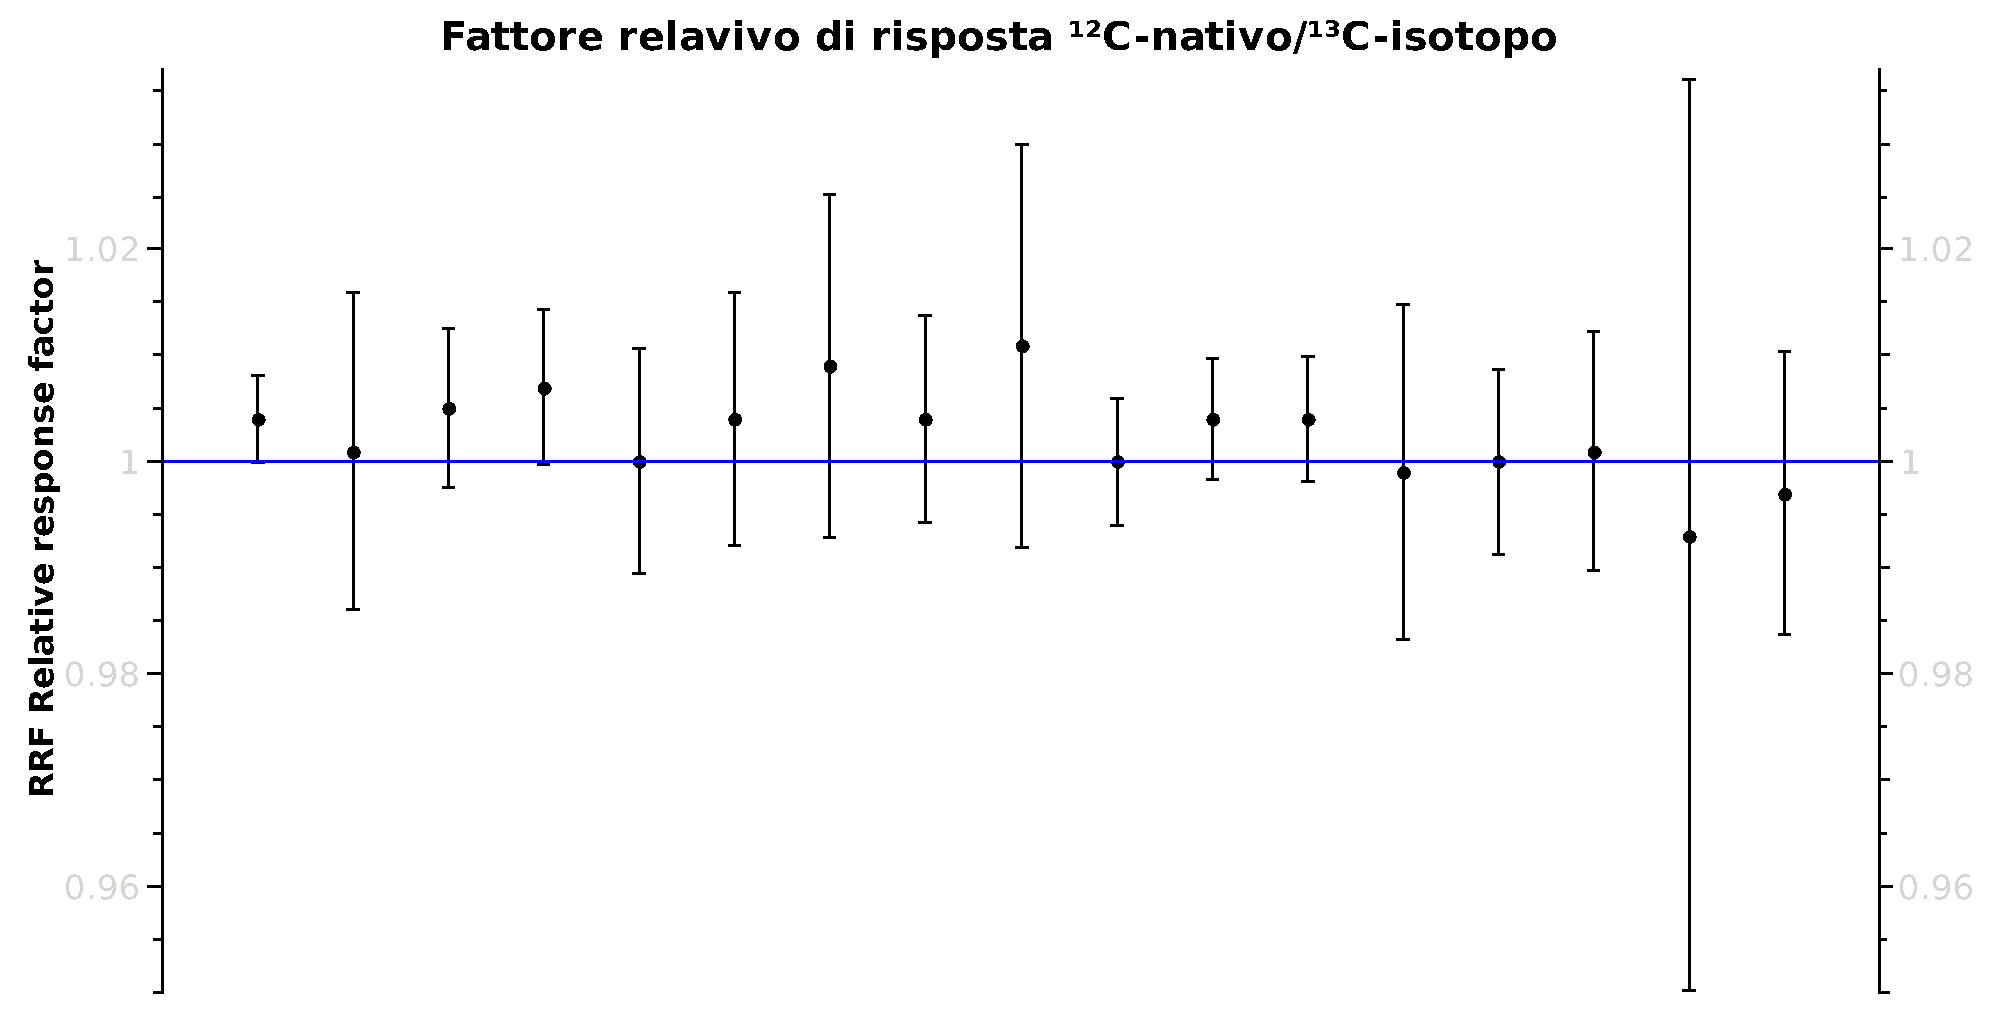
\includegraphics[width=1.04\textwidth]{img/2010-rrf.pdf}}}\end{figure}
\end{columns}

\end{frame}
\logo{
\includegraphics[width=0.1\paperwidth]{img/unipilogo.jpg}}

\subsubsection{Limiti di rivelabilità}\begin{frame}\frametitle{Validità di GC/MPI/TOF-MS: analisi di soluzioni arricchite}\framesubtitle{Limiti di rivelabilità}

I {\bf limiti di rivelabilità} di queste analisi sono risultati notevolmente bassi: \pause 
da 0.019pg a 0.43pg, in ogni caso {\bf minori dei LOD richiesti dallo standard JIS K0311} (0.1pg per i tetra e penta CDD e CDF; 0.2pg per gli esa e gli epta CDD e CDF; 0.5 per l'ottaCDD e l'ottaCDF).
\pause

Viene riportata una terza RSD dei RRF ed il coefficiente di determinazione $R^2$ della retta di calibrazione di cui però non viene riportato altro dato.

L'estremo del {\bf range lineare non è stato raggiunto} per restare sotto i limiti di concentrazione imposti dalla assicurazione della {\bf sicurezza}.

\end{frame}
\subsection{Validazione GC/MPI/TOF-MS: confronto con HRGC/HRMS}\subsubsection{Analisi di campioni di terreno contaminato}\begin{frame}\frametitle{Validazione GC/MPI/TOF-MS: confronto HRGC/HRMS}\framesubtitle{Analisi di campioni di terreno contaminato}


Sono stati analizzati {\bf 3 campioni di suolo inquinato} prelevati in una discarica di rifiuti industriali: verranno etichettati A, B e C. \pause {\bf Non viene riportata} la quantità di terreno estratto né la quantità di standard interno aggiunto (né se è stato aggiunto o se è stata impiegata una retta di calibrazione, né come è stato estratto e concentrato).\pause

I campioni {\bf sono stati estratti e lavati con due metodi differenti} per l'analisi GC/MPI/TOF-MS e HRGC/HRMS. Anche gli estratti hanno subito lavaggi differenti.

\begin{center}
   \begin{tabular}{c | c c}
& GC/MPI/TOF-MS & HRGC/HRMS \\
\hline
A & {\bf ASE} + veloce lavaggio & Soxhlet + fine lavaggio \\
B & {\bf ASE} + veloce lavaggio & Soxhlet + fine lavaggio  \\
C & {\bf Soxhlet} + veloce lavaggio &  Soxhlet + fine lavaggio 
   \end{tabular}
  \end{center}

\end{frame}
\logo{}
\subsubsection{Risultati dell'analisi di campioni di terreno contaminato}\begin{frame}\frametitle{Validazione GC/MPI/TOF-MS: confronto HRGC/HRMS}\framesubtitle{Risultati dell'analisi di campioni di terreno contaminato}
In figura sono riportate le {\bf differenze \% del metodo GC/MPI/TOF-MS rispetto al metodo HRGC/HRMS} per i tre campioni di suolo. Possiamo osservare che il campione C ha avuto dei recuperi più bassi {\bf  nonostante} l'estrazione con soxhelet.\pause

\vspace{10 pt}

\begin{columns}
\column{0.4\linewidth}
Vengono riportati anche i valori di TEQ e confrontati con quelli ottenuti per HRGC/HRMS. Nella tecnica GC/MPI/TOF-MS {\bf non sono stati analizzati gli altri composti partecipanti} (con fattori TEF minori) {\bf al TEQ} totale perciò si ottengono valori circa del 10\% inferiori.
\column{0.6\linewidth}\vspace{-10 pt}\begin{figure}{\centering{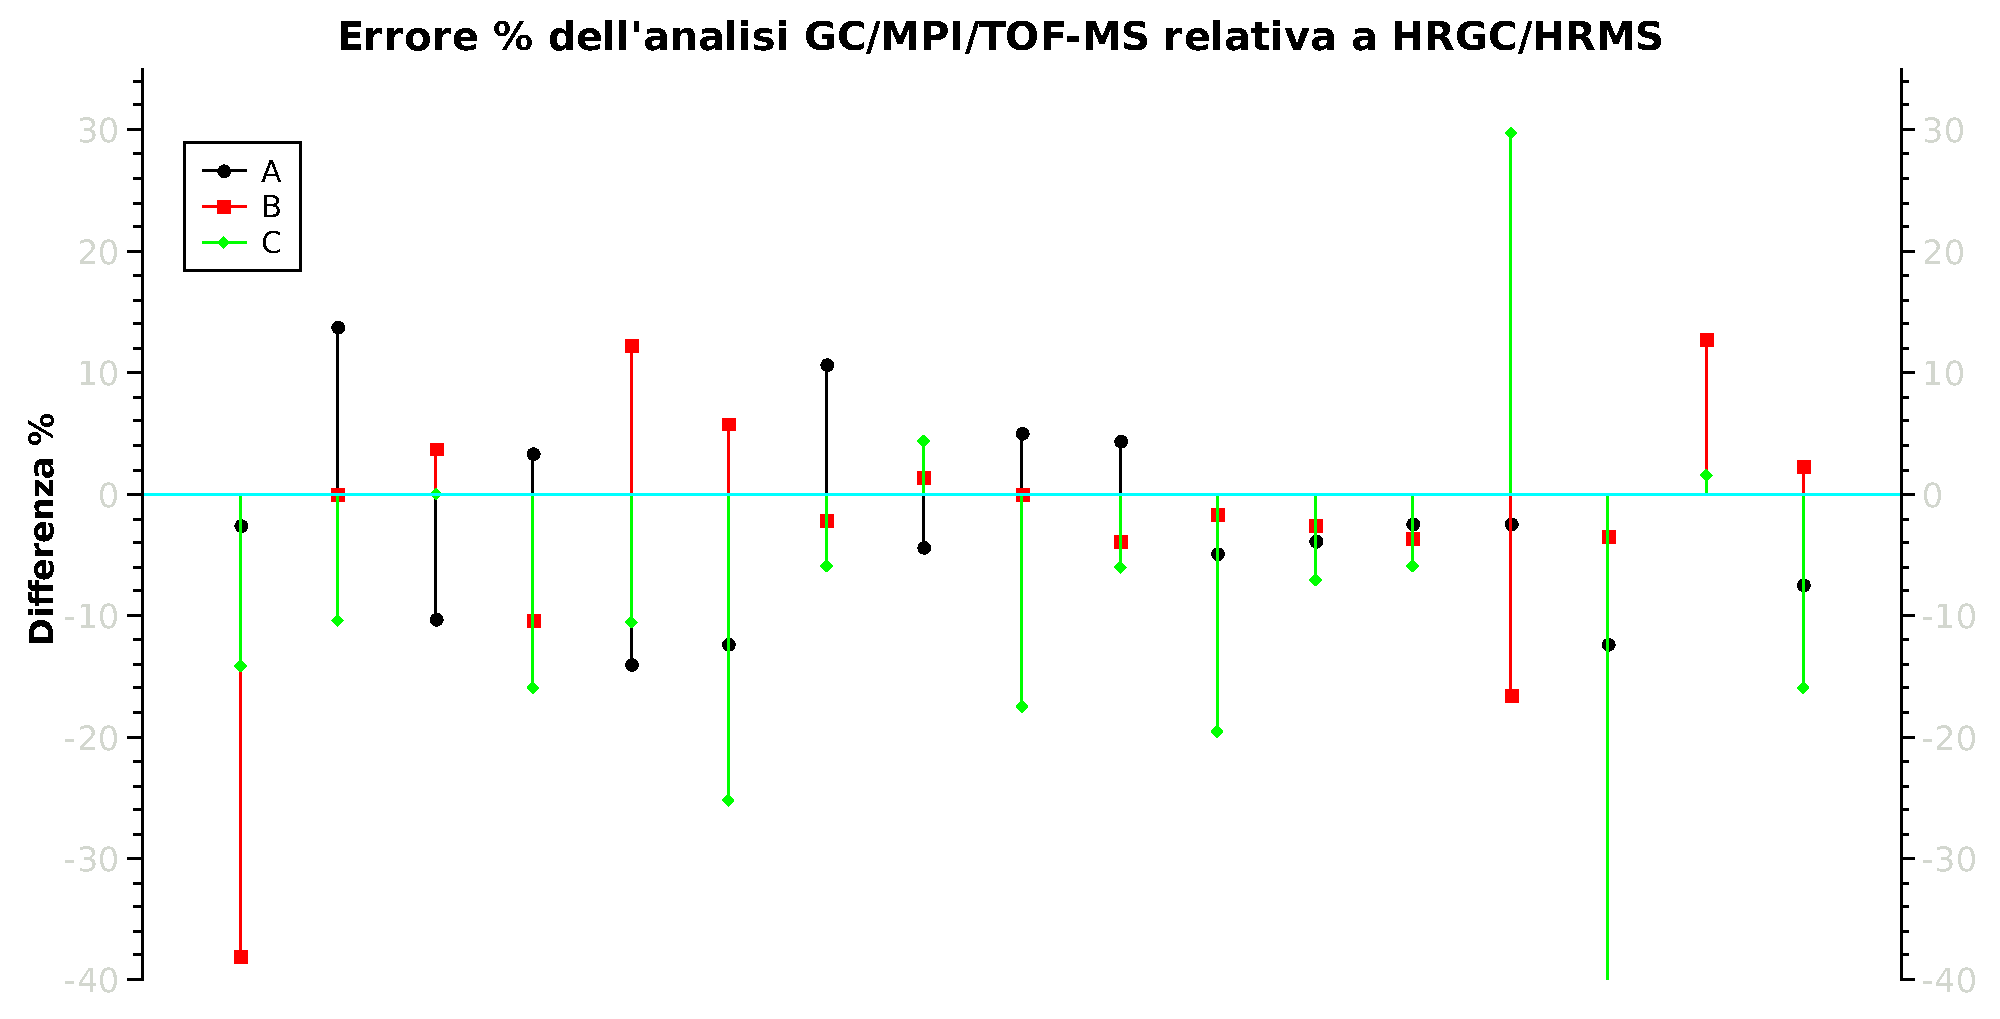
\includegraphics[width=1.03\textwidth]{img/errorediff.pdf}}}\end{figure}
\end{columns}
\end{frame}
\logo{
\includegraphics[width=0.1\paperwidth]{img/unipilogo.jpg}}
\subsection{Risultati dell'analisi di materiale certificato di terreno}\begin{frame}\frametitle{Risultati dell'analisi di materiale certificato di terreno}
È stato analizzato un campione di suolo di {\bf riferimento certificato} (JSAC0422). \pause L'estrazione viene effettuata seguendo la {\bf procedura veloce} e semplificata. Nella visualizzazione 2-D si osservano molti picchi non identificati ma i picchi precedentemente studiati si riescono ad identificare nuovamente. Lo stesso campione certificato viene analizzato anche con il metodo HRGC/HRMS con una procedura di lavaggio ed estrazione migliore. 

I valori di deviazione standard riportati nella tabella S-5 delle informazioni supplementari dell'articolo sono in realtà limiti di confidenza al 95\%.

Si osserva che i {\bf risultati ottenuti col metodo GC/MPI/TOF-MS sono migliori} rispetto a quelli ottenuti con HRGC/HRMS.

I risultati peggiori si ottengono per gli eptaCDD ed eptaCDF ed un tentativo di giustificazione si trova nell'articolo.
\end{frame}
\logo{}


\begin{frame}\frametitle{Risultati dell'analisi di materiale certificato di terreno}

\begin{figure}{\centering{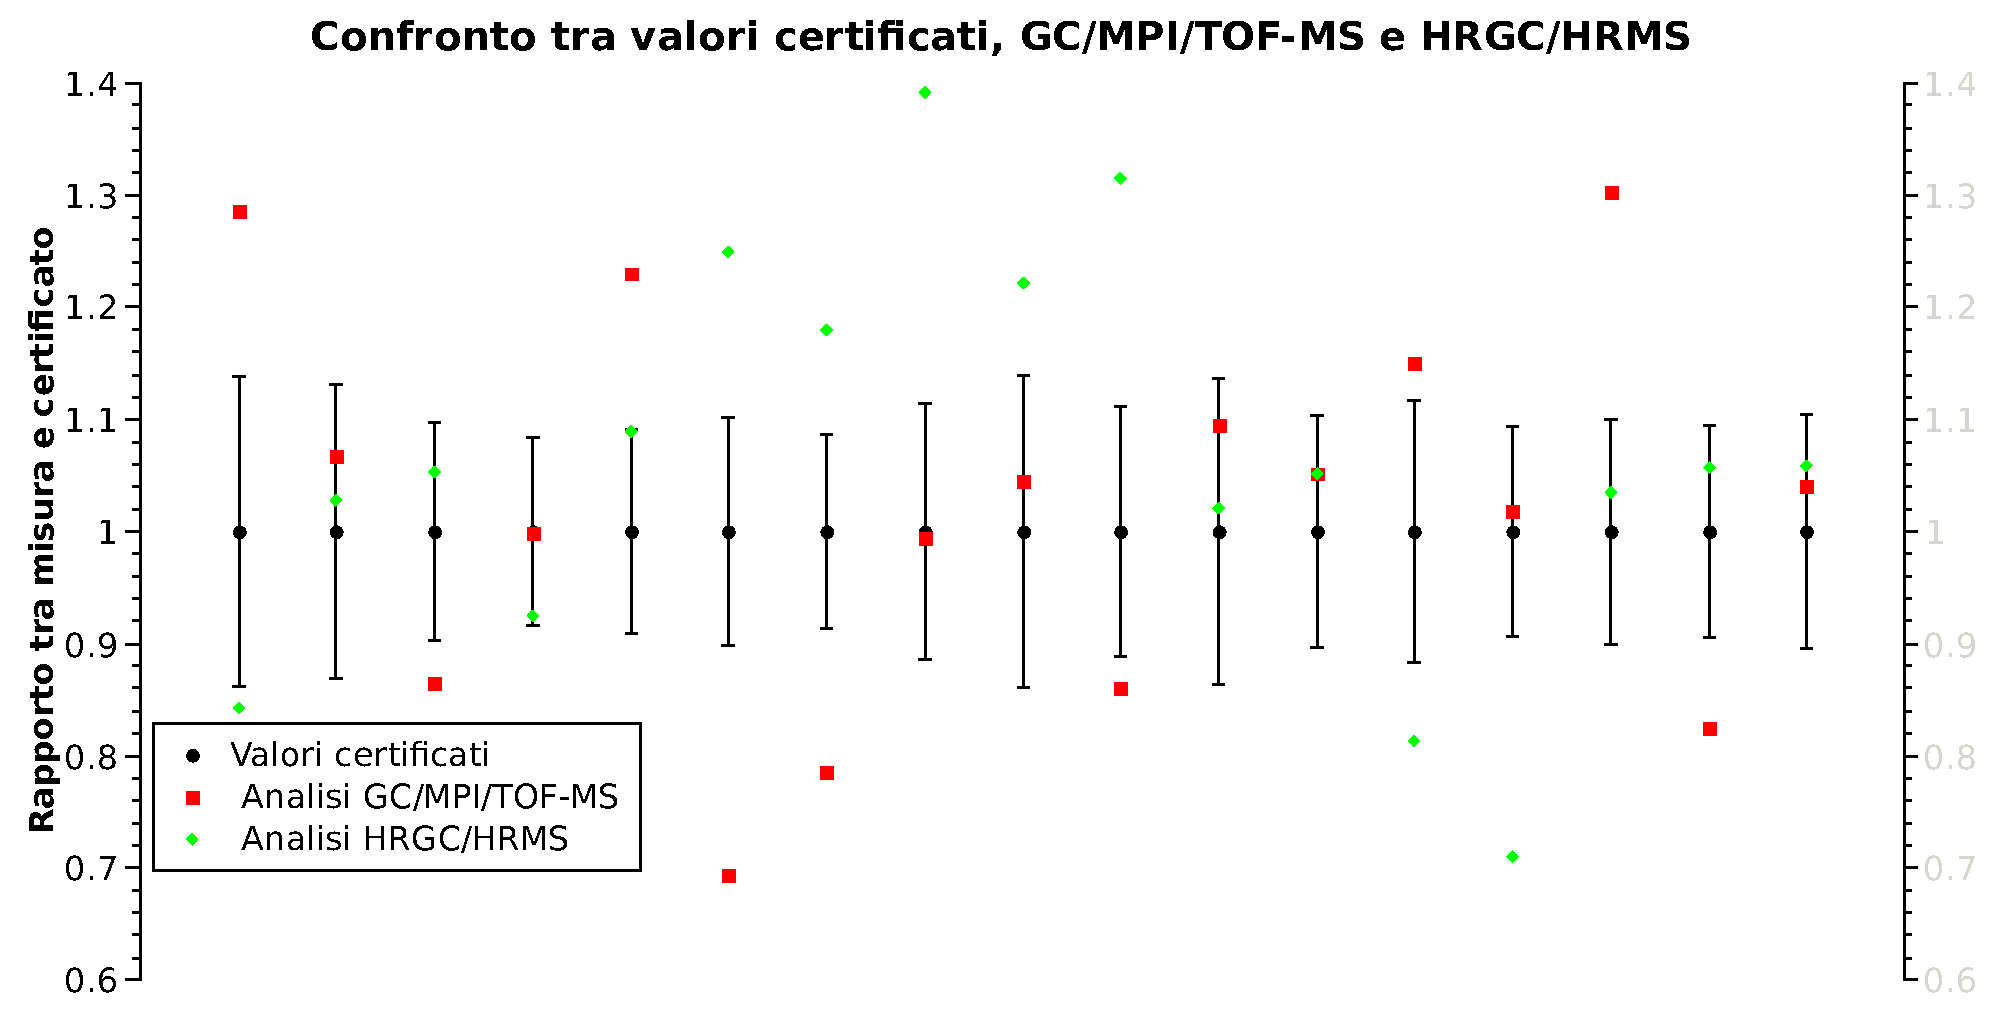
\includegraphics[width=1.04\textwidth]{img/SRM.pdf}}}\end{figure}

\end{frame}\logo{
\includegraphics[width=0.1\paperwidth]{img/unipilogo.jpg}}

\subsection{Conclusioni}\begin{frame}\frametitle{Conclusioni}

Sono state valutati i seguenti parametri:\begin{itemize}\pause
\item[\checkmark] esattezza rispetto ai valori ottenuti col metodo di riferimento,
\item[\checkmark] esattezza rispetto ai valori certificati nell'analisi di un SRM,
 \item[\checkmark] precisione,\pause
 \item[\checkmark] campo di applicazione ad altri analiti (sono state analizzate PCDD e PCDF mentre i PCB non si rivelano),
 \item[\checkmark] selettività in presenza di isomeri,\pause
 \item[\checkmark] più di un metodo di estrazione,\pause
 \item[\checkmark] limite di rivelabilità,
 \item[\checkmark] conformità ai parametri richiesti dallo standard nazionale,\end{itemize}
\end{frame}
\begin{frame}\frametitle{Conclusioni}
{\bf Non} sono state valutati i seguenti parametri:\pause\begin{itemize}
 \item[$\times$] robustezza,
 \item[$\times$] ottimizzazione,
 \item[$\times$] riproducibilità,
 \item[$\times$] incertezza,
 \item[$\times$] risultati dell'analisi sul bianco,
 \item[$\times$] valutazione dell'effetto matrice col metodo delle aggiunte,\pause
 \item[$\times$] range dinamico e lineare,\pause
 \item[$\times$] studi interlaboratorio,
 \item[$\times$] parametri di qualità e criteri di accettazione,
 \item[$\times$] recupero dello std. int. con i due metodi di estrazione e lavaggio,\pause
 \item[$\times$] campo di applicazione ad altre matrici (è stato testato solo terreno),\pause
 \item[$\times$] selettività in presenza di interferenti,\pause
 \item[$\times$] analisi critica dei risultati in disaccordo con il SRM.
\end{itemize}
\begin{center}
{\pause \huge FINE}
\end{center}
\end{frame}


